
\section{函数 $I(\cdot)$：从 $\Spec A$ 的子集到理想}

现在，我们引入一个概念，它在某种意义上是\trVanishingSet{}函数 $V(\cdot)$ 的
「逆」。给定 $\Spec A$ 的一个子集 $S$，$I(S)$ 是在 $S$ 上消失的那些函数所成的
集合；换言之，$I(S)=\bigcap_{[\mathfrak{p}]\in S}\mathfrak{p}\subset A$
（至少当 $S$ 非空时是如此）。

我们快速地作三条观察。（你能看出它们为什么都成立吗？）
\begin{itemize}
\item $I(S)$ 显然是 $A$ 的一个\trIdeal。
\item $I(\cdot)$ 反转包含关系：若 $S_1\subset S_2$，则 $I(S_2)\subset I(S_1)$。
\item $I(\overline{S})=I(S)$。
\end{itemize}

\begin{exercise}\label{ex:i-of-axis-and-point}
设 $A=k[x,y]$。若 $S=\{[(y)],\,[(x,y-1)]\}$（见图~\ref{fig:set-of-37a}），则
$I(S)$ 由那些在 $x$-轴上消失、并且在点 $(0,1)$ 处消失的多项式组成。试给出这个\trIdeal{}的生成元。
\end{exercise}

\begin{exercise}\label{ex:i-of-three-axes}
设 $S\subset\mathbb{A}^3_{\mathbb{C}}$ 是三条坐标轴的并。给出\trIdeal{} $I(S)$ 的生成元。务必给出证明！我们将在练习~13.1.F 中看到，这个\trIdeal{}无法由少于三个元素生成。
\end{exercise}

\begin{figure}[htbp]
\centering
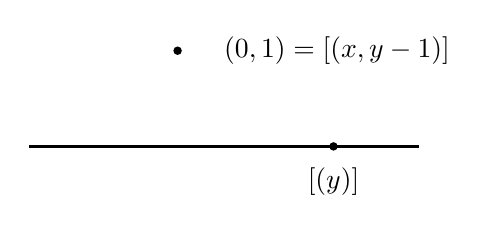
\begin{tikzpicture}[scale=0.9]
  \draw[thick] (-2.4,0) -- (3.1,0);
  \fill (1.9,0) circle (1.7pt) node[below=4pt] {$[(y)]$};
  \fill (-0.3,1.35) circle (1.7pt);
  \node at (1.95,1.35) {$(0,1)=[(x,y-1)]$};
\end{tikzpicture}
\caption{\cref{ex:i-of-axis-and-point} 的集合 $S$，画作 $\mathbb{A}^2$ 的一个子集。（依原书手绘图重绘。）}\label{fig:set-of-37a}
\end{figure}

\begin{exercise}\label{ex:v-of-i-is-closure}
证明 $V(I(S))=\overline{S}$。于是，当 $S$ 是\trClosedSet{}时，$V(I(S))=S$。
\end{exercise}

注意，$I(S)$ 总是一个\trRadicalIdeal——若 $f\in\sqrt{I(S)}$，则对某个 $n>0$，
$f^n$ 在 $S$ 上消失；于是 $f$ 在 $S$ 上消失，从而 $f\in I(S)$。

\begin{exercise}[容易的练习]\label{ex:i-of-v-is-radical}
证明：若 $J\subset A$ 是一个\trIdeal，则 $I(V(J))=\sqrt{J}$。（巨大的提示：\cref{ex:vanish-on-vi-radical}。）
\end{exercise}

\cref{ex:v-of-i-is-closure} 与 \cref{ex:i-of-v-is-radical} 表明，$V$ 与 $I$
是「差不多」互逆的。更精确地说：

\begin{theorem}\label{thm:closed-subsets-radical-ideals}
$V(\cdot)$ 与 $I(\cdot)$ 在 $\Spec A$ 的诸\trClosedSubset{}与 $A$ 的诸\trRadicalIdeal{}之间给出一个反转包含关系的双射（其中\trClosedSubset{}经 $I(\cdot)$ 给出\trRadicalIdeal，而\trRadicalIdeal{}经 $V(\cdot)$ 给出\trClosedSubset）。
\end{theorem}

\cref{thm:closed-subsets-radical-ideals} 有时被称为\trHilbert{}\trNullstellensatz，但我们把这个名字保留给 \cref{thm:hilbert-nullstellensatz}。

\begin{exercise}\label{ex:i-of-v-exceeds-j}
设 $J=(x^2+y^2-1,\,y-1)$。找出 $I(V(J))\smallsetminus J$ 中的一个元素，并给出证明。
\end{exercise}

\begin{exercise}[重要练习；参看\cref{ex:minimal-prime-ideals}]\label{ex:irreducible-prime-bijection}
证明：$V(\cdot)$ 与 $I(\cdot)$ 给出 $\Spec A$ 的\emph{\trIrreducible{}\trClosedSubset}与 $A$ 的\emph{\trPrimeIdeal}之间的一个双射。由此推证：$\Spec A$ 的点与 $\Spec A$ 的\trIrreducible{}\trClosedSubset{}之间存在双射（其中，一个点经取\trClosure{}确定一个\trIrreducible{}\trClosedSubset）。于是，\emph{$\Spec A$ 的每个\trIrreducible{}\trClosedSubset{}都恰有一个\trGenericPoint}——任何\trIrreducible{}\trClosedSubset{} $Z$ 都能唯一地写成 $\overline{\{z\}}$。
\end{exercise}

\begin{exercise}[练习兼定义]\label{ex:minimal-prime-ideals}
环 $A$ 的一个\trPrimeIdeal{}称为\textbf{\trMinimalPrimeIdeal{}}（minimal prime ideal）
（或者更简单些，\textbf{\trMinimalPrime{}}（minimal prime）），如果它在包含关系之下是极小的。（例如，$k[x,y]$ 的唯一\trMinimalPrimeIdeal{}是 $(0)$。）设 $A$ 是任意的环，证明 $\Spec A$ 的\trIrreducibleComponent{}与 $A$ 的\trMinimalPrimeIdeal{}之间存在双射。特别地，$\Spec A$ 是\trIrreducible{}的，当且仅当 $A$ 只有一个\trMinimalPrimeIdeal{}；这推广了\cref{ex:integral-domain-irreducible}。
\end{exercise}

命题~3.6.15、\cref{ex:noetherian-ring-spec-noetherian} 与 \cref{ex:minimal-prime-ideals} 蕴含：每个\trNoether{}环都只有有限多个\trMinimalPrimeIdeal{}。一个代数事实，如今被揭示出来：它其实是一个「几何」事实！

\begin{exercise}[现实检验]\label{ex:irreducible-factors-components}
在 $\mathbb{A}^n_k=\Spec k[x_1,\dots,x_n]$ 中，由 $f(x_1,\dots,x_n)\in k[x_1,\dots,x_n]$ 切出的子集，理应具有一些\trIrreducibleComponent{}，与 $f$ 的互不相同的\trIrreducible{}因子相对应。证明这一点。（环 $k[x_1,\dots,x_n]$ 的什么性质使这件事得以成立？）
\end{exercise}

\begin{exercise}\label{ex:minimal-primes-quotient-xy}
$k[x,y]/(xy)$ 的\trMinimalPrimeIdeal{}是什么（其中 $k$ 是一个\trField）？
\end{exercise}

\textbf{3.7.2.\ 代数与几何之间一部宏大词典的开端。}\quad 我们此刻已在编纂一部代数与几何之间的宏大词典的路上行进了很远；随着理解的日益加深，你应当不断为这张表增补词条。

\begin{table}[htbp]
  \centering
  \footnotesize
  \begin{tabular}{|>{\raggedright\arraybackslash}p{5.6cm}|>{\raggedright\arraybackslash}p{5.2cm}|>{\raggedright\arraybackslash}p{2.6cm}|}
    \hline
    代数 & 几何 & 参看 \\
    \hline
    \trRing{} $A$ & \trAffineScheme{} $\Spec A$ & \mbox{\S3.2.1} \\
    \hline
    $\mathfrak{p}=I(\mathfrak{p})$：$A$ 的\trPrimeIdeal & $\mathfrak{p}=[\mathfrak{p}]$：$\Spec A$ 的点 & \mbox{\S3.2.1}、\mbox{\S3.7} \\
    \hline
    元素 $f\in A$ & $\Spec A$ 上的函数 $f$ & \mbox{\S3.2.1} \\
    \hline
    $f\pmod{\mathfrak{p}}$ & $f(\mathfrak{p})$；函数 $f$ 在 $\mathfrak{p}$ 处的值 & \mbox{\S3.2.1} \\
    \hline
    $f\in\mathfrak{p}$ & 函数 $f$ 在 $\mathfrak{p}$ 处消失（为零） & \mbox{\S3.2.1} \\
    \hline
    $A$ 的\trNilradical{}理想 $\mathfrak{N}=\sqrt{(0)}=\bigcap\mathfrak{p}$ & 在每一点处都消失的函数 & \mbox{\cref{thm:nilradical-intersection-primes}} \\
    \hline
    $A$ 的\trMaximalIdeal & $\Spec A$ 的作为点的\trIrreducible{}\trClosedSubset{}（即 $\Spec A$ 的\trClosedPoint） & \mbox{练习~3.6.I} \\
    \hline
    $\mathfrak{p}=I(Z)$：$A$ 的\trPrimeIdeal（又一次！） & $\Spec A$ 的\trIrreducible{}\trClosedSubset{} $Z=V(\mathfrak{p})$ & \mbox{\cref{ex:irreducible-prime-bijection}} \\
    \hline
    $A$ 的\trMinimalPrimeIdeal{} & $\Spec A$ 的\trIrreducibleComponent{} & \mbox{\cref{ex:minimal-prime-ideals}} \\
    \hline
    $A$ 的\trRadicalIdeal{} $I=\sqrt{I}=I(S)$ & $\Spec A$ 的\trClosedSubset{} $S=V(I)$ & \mbox{\cref{thm:closed-subsets-radical-ideals}} \\
    \hline
  \end{tabular}
\end{table}
